\section{CAN Bus}

\subsection{CAN Geschichte}
	
Das Controller Area Network ist ein serielles Bus System und wurde
1983, zur Vernetzung von Steuergeräten in Automobilen, von der Firma
Bosch GmbH entwickelt. Doch nicht nur in der Automobilindustrie,
sondern auch in der Medizintechnick, Flug- und Raumfahrttechnik sowie
in Aufzuganlagen und im Schiffsbau, kann man auf einen CAN Bus stoßen
\citep[nach][]{WI1}. Der Vorteil gegüber der herkömmlichen Verkablung
lag darin, das mehrere Knoten über dieselbe Leitung Kommunizieren
können. Alle Teilnehmer können Pakete priorisiert mit
Kollisionserkennung auf den Bus legen, hierbei wird die Nachricht,
nicht der Empfänger adressiert.
	
\subsection{Busankoplung/Vernetzung von CAN-Knoten}
	
\subsection{CAN-Bus Pegel} Beim CAN-Bus erfolgt die Übertragung der
Bits über 2 Pegel: 
\begin{itemize} 
\item Dominant 
\item Rezessiv
\end{itemize}

Wenn beide Pegel gleichzeitig gesendet werden, so überschreibt immer
der dominante Pegel den rezessiven Pegel.
	
\subsection{Bit Stuffing} 
Bit-Stuffing beim CAN-Bus bedeutet, dass
nach 5 Bits mit gleichem Pegel ein ">Stuff Bit"< mit inversem Pegel
eingefügt wird. Die Empfänger filtern diese Stuff-Bits, dann nach dem
gleichen Schema wieder heraus.
\\ Bit stuffing wird einerseits
eingesetzt, weil Bitfolgen mit mehr als 5 Bits mit gleichem Pegel für
Steuerungszwecke eingesetzt werden, und andererseits auch wegen der
NRZ-Kodierung. Das heißt dass der Pegel bei zB 4 rezessiven Bits
gleich bleibt. Wenn dann beispielsweise 10 gleiche Bits übertragen
werden, so kann der Empfänger möglicherweise nicht mehr unterscheiden,
ob jetzt 10 oder 11 Bits übertragen wurden.
	
\subsection{CAN Frames} Beim CAN-Bus gibt es 4 unterschiedliche Arten
von Frames: 
\begin{itemize} 
\item Daten-Frame 
\item Remote-Frame 
\item Error-Frame 
\item Overload-Frame 
\end{itemize} 

\subsubsection{Daten Frame} 
Die Daten-Frames dienen dem Transport von Daten und können bis
zu 8 Byte an Nutzdaten enthalten. Bei den Daten-Frames kann zwischen
Standard Format und Extended Format unterschieden werden, die sich
hauptsächlich in der Länge des Identifiers unterscheiden. Der Aufbau
eines Daten Frames kann aus Abbildung \ref{data} entnommen werden.
	
\begin{figure}[htbp] 
\centering
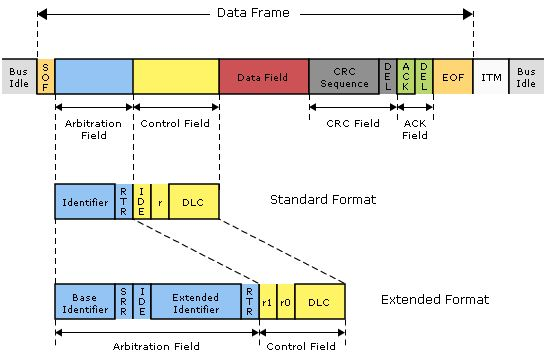
\includegraphics[width=0.7\textwidth]{figures/data-frame}
\caption{Aufbau eines Daten-Frames \citep{HYC}} 
\label{data}
\end{figure} 
%Quelle: http://marco.guardigli.it/2010/10/hacking-your-car.html
		
Gestarted wird ein Frame durch das \textbf{SOF} (start-of-frame)
bestehend aus einem dominanten Bit. Darauf folgt gleich das
Arbitrationsfeld und dem Kontrollfeld. Abhängig vom Format bestehen
diese aus \textbf{Basis Identifier} (11 Bits), \textbf{Extended
Identifier} (18 Bit), einem \textbf{RTR}-Bit (remote transmission
request; bei Remote-Frames rezessiv) sowie einem \textbf{SRR}-Bit
(substitude-remote-request; rezessiv). Ist das \textbf{IDE}-Bit
(identifier extension) rezessiv, so handelt es sich um das Extended
Format, das somit immer Nachrang über dem Standard Format hat.\\ Im
Kontrollfeld befindet sich neben 1-2 reservierten (aktuell nicht
verwendeten) Bits der aus 4 Bits bestehende \textbf{DLC} (data length
code), der die Länge des nachfolgenden \textbf{Datenfeldes} angibt.\\
Wie bereits erwähnt können mit den Daten-Frames bis zu 8 Byte, also 64
Bit, übertragen werden. dies kann jedoch nur in einheiten von 8 Bits
geschehen. Anschließend an das Datenfeld ist das CRC-Feld (cyclic
redundancy check; Prüfsummenfeld) bestehend aus 16 Bit (15 Bit + 1
rezessives Delimiter-Bit). Des weiteren enthält ein Daten-Frame ein
\textbf{ACK}-Feld (Acknowledge). Dieses wird verwendet, um den Empfang
eines korrekten Frames zu bestätigen. Der Sender sendet dafür ein
rezessives Bit. Jeder Empfänger der keinen Fehler feststellen konnte,
setzt einen dominanten Pegel und überschreibt somit den rezessiven des
Senders. Im Falle einer negativen Quittierung (rezessiver Pegel) muss
der Knoten, der den Fehler erkannt hat, nach dem ACK-Delimiter einen
Error-Frame aussenden.\\Das Ende des Frames wird mit 7 rezessiven Bits
dem \textbf{EOF} (end of frame) angezeigt. Anschließend an den Frame
muss ein ITM-Package (intermission oder inter-frame-space) bestehend
aus mindestens 3 rezessiven Bits gesendet werden.
	
\subsubsection{Remote Frame} Mit Hilfe der Remote-Frames können
Daten-Frames von anderen Teilnehmern angefordert werden. Der Frame
unterscheidet sich vom Daten-Frame durch ein rezessives Bit im
">RTR"<-Slot, wodurch Remote-Frames im Falle einer Kollision immer
Nachrang gegenüber den Daten-Frames haben, und durch ein Fehlen des
Datenfeldes.
	
\subsubsection{Error Frame} Erkennt ein CAN-Knoten einen Fehler, so
sendet er einen Error-Frame an alle anderen CAN-Knoten im Netzwerk.
Bei diesen Frames wird das Bit-Stuffing bewusst ignoriert. Der
Error-Frame besteht aus 2 Feldern, den Error-Flags und dem
Error-Delimiter (8 rezessive Bits). Die Error-Flags sind abhängig vom
Modus in dem sich ein CAN-knoten befindet. Ist der Knoten im
Fehler-Status \textit{">error active"<} so setzt er die Error-Flags
auf 6 dominante Bits. Befindet er sich hingegen im Fehler-Status
\textit{">error passive"<} so sendet er 6 rezessive Bits.
	
\subsubsection{Overload Frame} Overload-Frames werden als Zwangspause
zwischen Daten- und Remote-Frames genutzt. Dabei hat ein
Overload-Frame das gleiche Format wie ein Active-Error-Frame. Wie in
Abbildung \ref{overload} ersichtlich ist, besteht der Overload-Frame
ebenfalls aus 2 Feldern: dem Overload-Flag (6 dominante Bits) und dem
Overload-Delimiter (8 rezessive Bits). Ein Overload-Frame kann jedoch
nur während eines Interframespaces gesendet werden. Dies ermöglicht
die Unterscheidung von den Error-Frames, die während der Übertragung
einer Nachricht gesendet werden, sobald eben ein Fehler erkannt wurde.

	
\begin{figure}[htbp] 
\centering
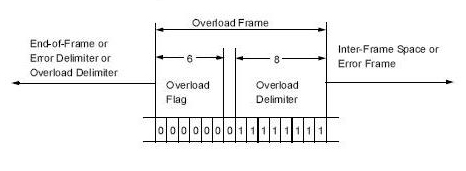
\includegraphics[width=0.7\textwidth]{figures/overload-frame}
\caption{Aufbau eines Overload-Frames \citep{CBM}} 
\label{overload}
\end{figure} 
% Quelle: http://rs232-rs485.blogspot.co.at/2009/11/can-bus-message-frames-overload.html
	
	\subsection{Zeichenkodierung}
	
	\subsection{Bit-Timing}
	
	\subsection{Synchronisatzion}
	
	\subsection{Buszugriffsverfahren}
	
	\subsection{Fehlermanagement}
	
	\subsection{Sicherungsmechanismen/Fehlererkennung}

\section{CAN Bus over Ethernet}
	
	\subsection{Probleme}
	
	\subsection{Bestehende Lösungen}



\newpage \addcontentsline{toc}{section}{Abbildungen} \listoffigures

\newpage \addcontentsline{toc}{section}{Literatur}
\bibliographystyle{abbrv} 
%\bibliographystyle{alphadin}
\bibliography{quellen}
